% instead of amberg, the option weiden oder amwen can be given. This changes the title backround
% lecture argument adds the subtitle to the footline
% other formats possible, e.g. aspectratio=43 or aspectration=169
\documentclass[aspectratio=169, lecture, amberg]{OTHAWbeamer}
\let\Tiny=\tiny

\usepackage{etex}
\usepackage{graphicx}
\usepackage{xcolor}
\usepackage{hyperref}
\usepackage{booktabs}
\usepackage[utf8]{inputenc}
\usepackage[ngerman, english]{babel}
\usepackage[
backend=biber,
style=ieee,
sorting=none
]{biblatex}

\title[Action Spotting with UGL]{Unifying Global and Local Features}
\subtitle{A Modern Approach to Sports Video Analysis}
\author[Presenter]{Hieu Tran}
\place{Amberg}
\date{\selectlanguage{english}\today}

\addbibresource{literature.bib}

\begin{document}
\maketitle

\begin{frame}
\frametitle{\textbf{Table of Content}}
\setcounter{tocdepth}{1}
\setbeamerfont{section in toc}{series=\bfseries}
\setbeamertemplate{section in toc}[sections numbered]
\tableofcontents
\end{frame}

\section{Introduction}

\begin{frame}
\frametitle{1. Introduction}
\framesubtitle{Task Overview}
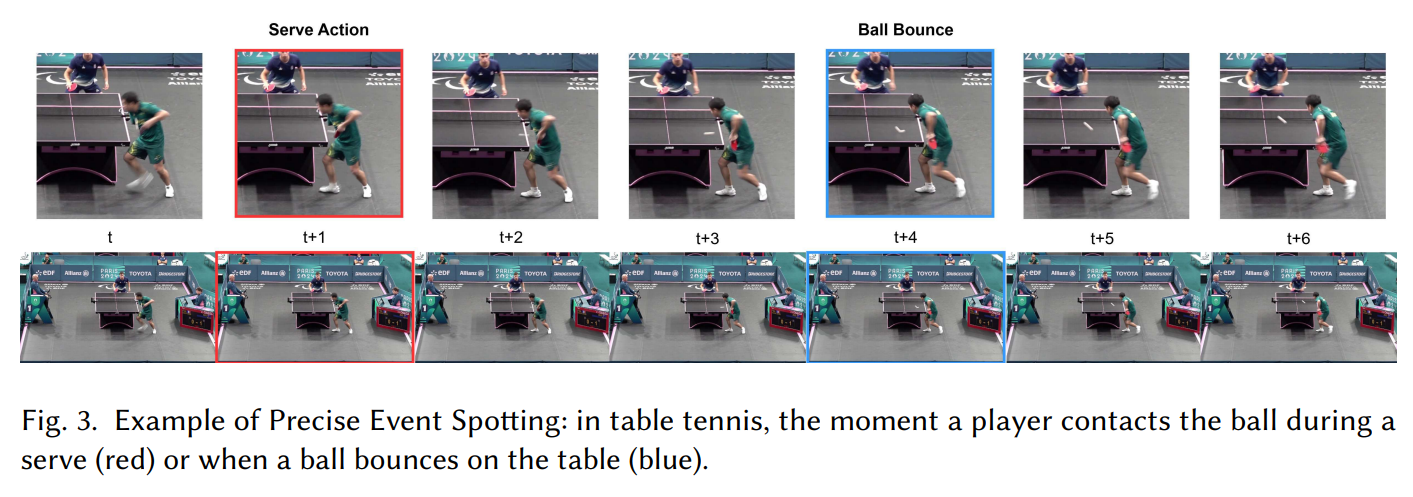
\includegraphics[width=0.95\textwidth,height=5.5cm]{images/intro.png}
\vspace{0.25cm}
\begin{flushright}
\tiny\textcolor{gray}{Xu H, Baniya AA, Well S, Bouadjenek MR, Dazeley R, Aryal S. Deep Learning for Sports Video Event Detection: Tasks, Datasets, Methods, and Challenges. arXiv:2505.03991, 2025.}
\end{flushright}
\end{frame}

\begin{frame}
\frametitle{1. Introduction}
\framesubtitle{Task Overview}
\begin{itemize}
\item<1-> \structure{Domain}: Action spotting in sports videos (soccer, diving, gymnastics)
\item<2-> \structure{Goal}: Detect \textit{precise timestamps} of events, not long temporal segments
\item<3-> \structure{Applications}: 
	\begin{itemize}
	\item Highlight generation
	\item Video analytics and broadcasting automation
	\item Downstream temporal retrieval
	\end{itemize}
\end{itemize}
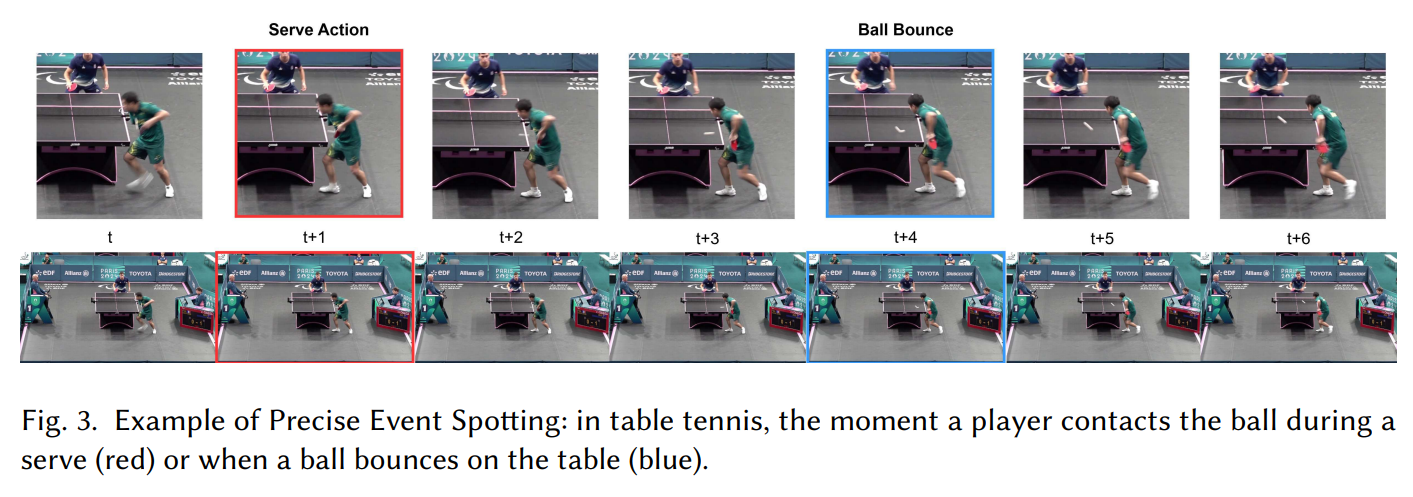
\includegraphics[width=0.55\textwidth,height=3.5cm]{images/intro.png}
\vspace{0.1cm}
\begin{flushright}
\tiny\textcolor{gray}{Xu H, Baniya AA, Well S, Bouadjenek MR, Dazeley R, Aryal S. Deep Learning for Sports Video Event Detection: Tasks, Datasets, Methods, and Challenges.}
\end{flushright}
\end{frame}

\begin{frame}
\frametitle{1. Introduction}
\framesubtitle{Motivation for UGL}
\begin{itemize}
\item<1-> Standard pipelines rely on \structure{global frame features} only
\item<2-> Current methods behave as black boxes, missing small but critical entities
\item<3-> Two-phase approaches: heavy 3D backbones, multiple extractors
\item<4-> End-to-end methods (e.g., E2E-Spot): lighter but still global-only
\end{itemize}
\end{frame}

\section{UGL Architecture}

\subsection{Global Environment Feature}


\begin{frame}
\frametitle{2. UGL Architecture}
\framesubtitle{Global Environment Feature}
\centering
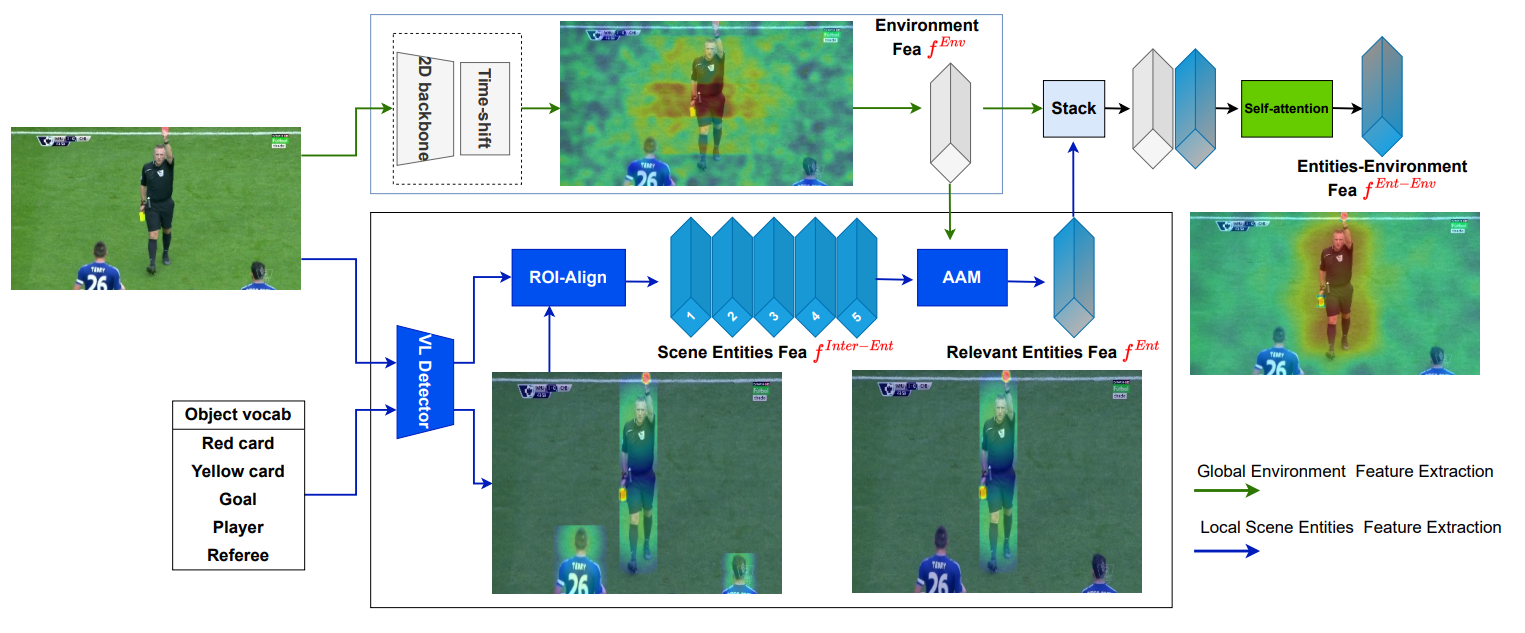
\includegraphics[width=1\textwidth,height=5.5cm]{images/architect.png}
\end{frame}


\subsection{Global Environment Feature}

\begin{frame}
\frametitle{2. UGL Architecture}
\framesubtitle{Global Environment Feature}
\begin{itemize}
\item<1-> \structure{Backbone}: RegNet-Y (efficient 2D CNN design)
\item<2-> \structure{Temporal Integration}: Gate-Shift Module (GSM)
	\begin{itemize}
	\item Shifts feature maps forward and backward along temporal axis
	\item Shares information across frames
	\item Lightweight alternative to 3D CNNs
	\end{itemize}

\item<3-> \structure{Output}: Global environment feature vector per frame capturing spatial and short-term temporal context
\end{itemize}
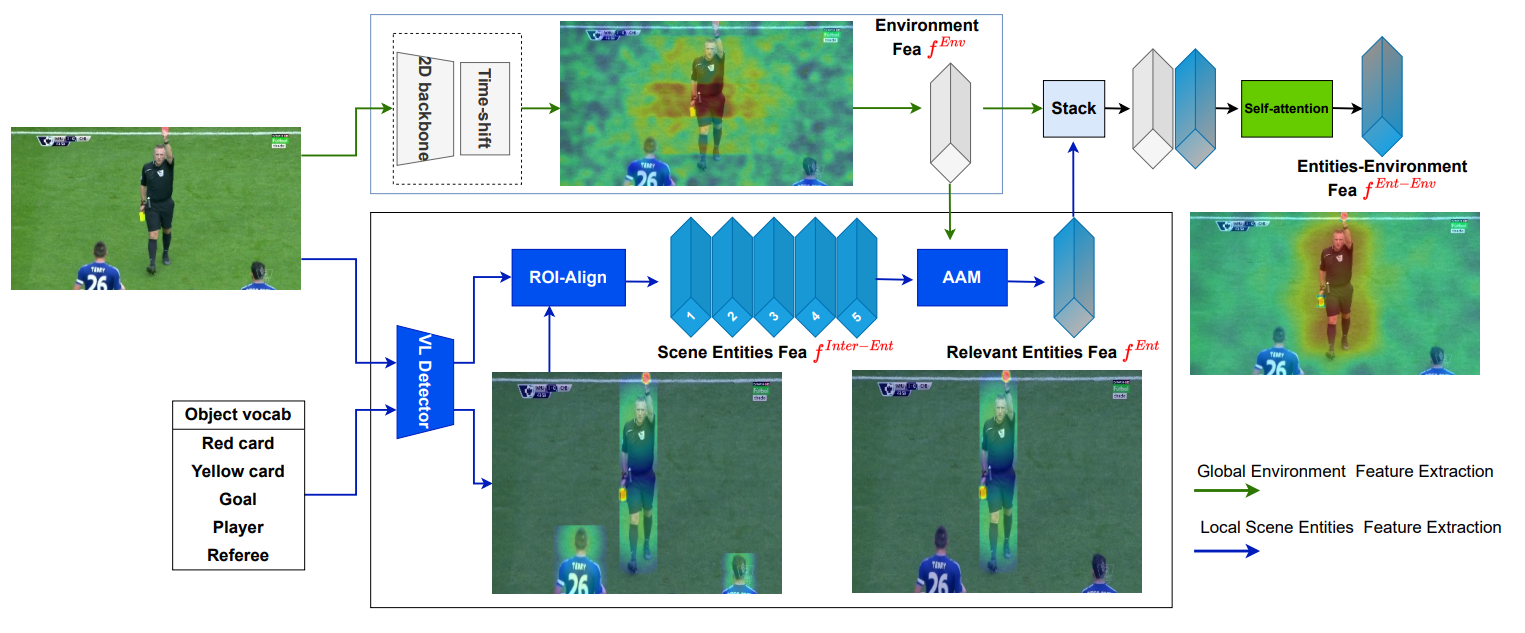
\includegraphics[height=3.5cm]{images/architect.png}
\end{frame}

\subsection{Local Scene Entities}

\begin{frame}
\frametitle{2. UGL Architecture}
\framesubtitle{Local Scene Entities with GLIP}
\begin{block}{Why GLIP?}
Global features alone often ignore small but crucial entities (cards, ball, etc.), especially under class imbalance
\end{block}

\begin{itemize}
\item \structure{GLIP}: Grounded Language-Image Pre-training (training-free detector)
\item \structure{Input}: Frame image + text prompt listing sports entities
	\begin{itemize}
	\item \textit{``ball, yellow card, red card, referee, \ldots''}
	\end{itemize}
\item \structure{Mechanism}: 
	\begin{itemize}
	\item Language encoder processes text (BERT)
	\item Visual encoder produces image proposals (Swin backbone)
	\item Cross-modal multi-head attention aligns proposals with textual entities
	\end{itemize}
\end{itemize}
\end{frame}

\begin{frame}
\frametitle{2. UGL Architecture}
\framesubtitle{Adaptive Attention Mechanism (AAM)}
\begin{block}{Problem}
Not all detected entities are equally relevant for the current action
\end{block}

\begin{block}{AAM Solution}
Takes both local entity features and global environment feature:
\begin{enumerate}
\item \structure{Hard attention}: Select most promising entities
\item \structure{Soft self-attention}: Fuse them into single compact representation
\end{enumerate}
\end{block}

\begin{block}{Output}
\structure{Local relevant scene entities feature} emphasizing objects crucial for the action
\end{block}
\end{frame}

\begin{frame}
\frametitle{2. UGL Architecture}
\framesubtitle{Fusion of Global and Local}
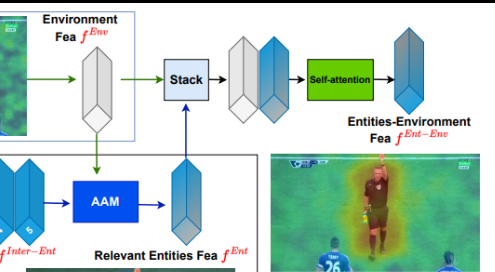
\includegraphics[height=6cm]{images/fusion.png}
\end{frame}

\begin{frame}
\frametitle{2. UGL Architecture}
\framesubtitle{Fusion of Global and Local}
\begin{enumerate}
\item<1-> \structure{Concatenate}:
	\begin{itemize}
	\item Global environment feature
	\item Local relevant entities feature
	\end{itemize}
\item<2-> \structure{Apply}:
	\begin{itemize}
	\item Self-attention layer to model interactions
	\item Average pooling for compactness
	\end{itemize}
\item<3-> \structure{Output}: Unified entities and environment representation per frame capturing both background context and key object semantics
\end{enumerate}
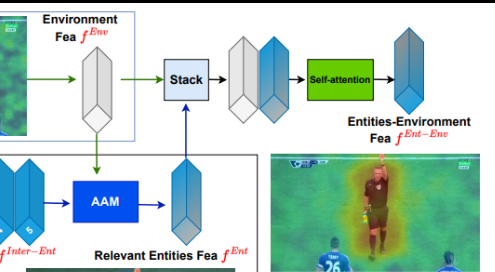
\includegraphics[scale=0.25, keepaspectratio]{images/fusion.png}
\end{frame}

\subsection{Temporal Reasoning}

\begin{frame}
\frametitle{2. UGL Architecture}
\framesubtitle{Long-Term Temporal Reasoning (LTR)}
\centering
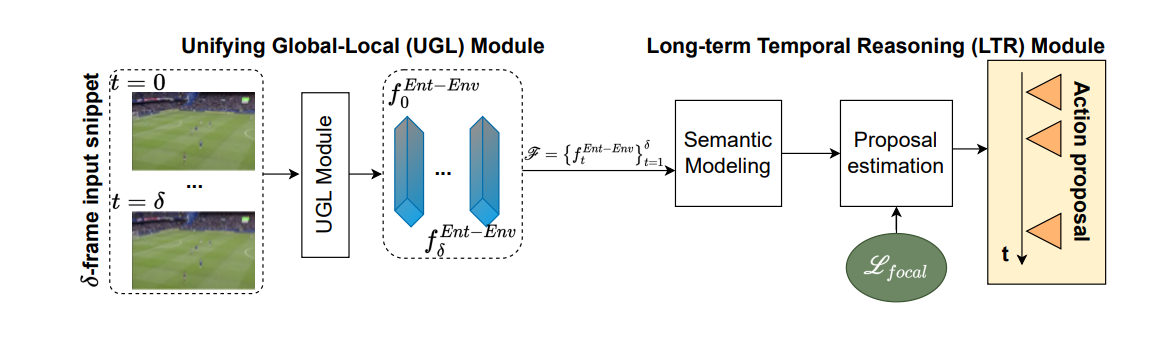
\includegraphics[width=0.85\textwidth,height=6cm]{images/ltr.png}
\end{frame}

\begin{frame}
	\frametitle{2. UGL Architecture}
	\framesubtitle{Long-Term Temporal Reasoning (LTR)}
	\begin{block}{Temporal Modeling}
		\begin{itemize}
			\item Input: Sequence of fused frame features for $T$-frame snippet
			\item Model: 1-layer \textbf{bidirectional GRU} capturing semantic relationships
			\item Prediction: Per-frame class scores via fully connected + softmax
		\end{itemize}
		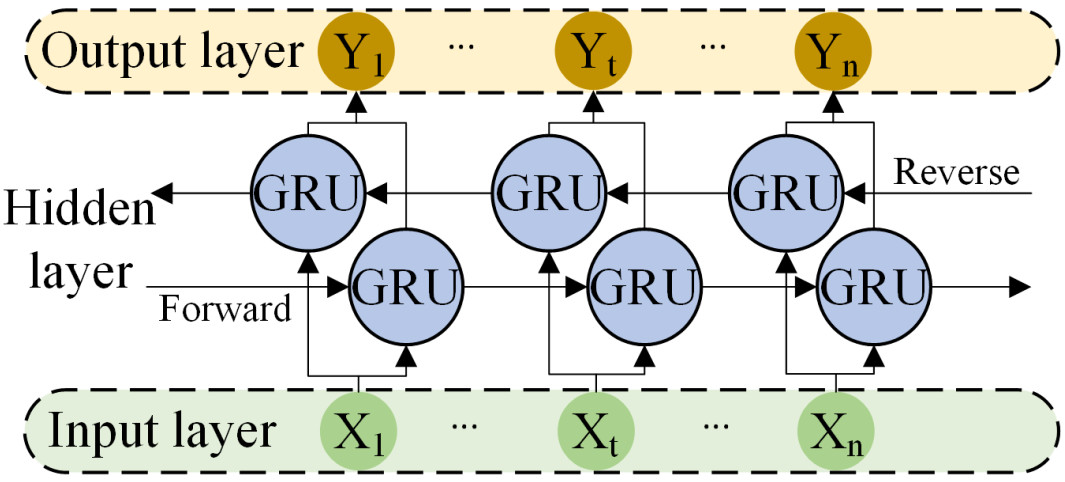
\includegraphics[width=0.55\textwidth,height=3cm]{images/biGRU.jpg}
		% Intelligent prediction of rail corrugation evolution trend based on self-attention bidirectional TCN and GRU
		% Jian-Hua Liu, ... Wei-Wei Yang
			\vspace{0.25cm}
			\begin{flushright}
			\tiny\textcolor{gray}{Liu JH, Yang WH, He J, Wang ZM, Jia L, Zhang CF, Yang WW. Intelligent prediction of rail corrugation evolution trend based on self-attention bidirectional TCN and GRU. Intell. Robot. 2024;4(4):318--338.}
			\end{flushright}
\end{block}
\end{frame}

\section{Benchmark Datasets}
\begin{frame}
\frametitle{3. Benchmark Datasets}
\framesubtitle{Three Sports Domains}
\begin{columns}
\begin{column}{0.5\textwidth}
\structure{SoccerNet-v2}
\begin{itemize}
\item $\sim$550 matches
\item $\sim$764 hours of video
\item $>$300k labeled spots
\item Strong clutter, camera changes
\end{itemize}

\structure{FineDiving}
\begin{itemize}
\item 3,000 diving clips
\item Phase transitions (entry, twist, etc.)
\end{itemize}
\end{column}
\begin{column}{0.5\textwidth}
\structure{FineGym}
\begin{itemize}
\item 5,374 gym performances
\item 32 spotting classes
\item Converted from action segments to timestamps
\end{itemize}
\end{column}
\end{columns}
\end{frame}


	\section{Quantitative Results}
\subsection{Evaluation Metrics}

\begin{frame}
\frametitle{4. Quantitative Results}
\framesubtitle{SoccerNet-v2; FineDiving \& FineGym}

\begin{table}[ht]
\centering
\caption{SoccerNet-v2 challenge quantitative comparison (T-mAP).}\label{tab:soccernet_results}
\begin{tabular}{lccc}
\toprule
Method & T-mAP (\%) & Gap to UGL (\%) & Notes \\
\midrule
UGL (ours) & \textbf{69.38} & -- & current SOTA \\
E2E-Spot & 66.73 & -2.65 & previous SOTA \\
Soares (two-phase) & 67.81 & -1.57 & 1st 2022\\
\bottomrule
\end{tabular}
\end{table}

\vspace{0.4cm}

\begin{table}[ht]
\centering
\caption{FineDiving and FineGym improvements of UGL over E2E-Spot (no optical flow).}\label{tab:finediving_finegym_results}
\begin{tabular}{lcc}
\toprule
Dataset & $\Delta$ mAP (Gap to E2E-Spot) (\%) \\
\midrule
FineDiving & 87.7 (+2.4) \\
FineGym & 67.8 (+1.3) \\
\bottomrule
\end{tabular}
\end{table}

\end{frame}

\section{Conclusion}

\begin{frame}
\frametitle{5. Conclusion}
\begin{itemize}
	\item Global + Local entity features to produce precise, interpretable per-frame representations
	\item Top result on SoccerNet‑v2: \textbf{69.38\% T‑mAP} 
	\item GRU + Focal Loss handles temporal reasoning and class imbalance effectively
\end{itemize}
\end{frame}

\begin{frame}
\centering
\vfill
{\LARGE Thank you for listening!}\\[1em]
{\large Questions are welcome}
\vfill
\end{frame}

\appendix

\section{Appendix}

\begin{frame}
\frametitle{Appendix }
\framesubtitle{A. Gate-Shift Module}
\begin{itemize}
\item \structure{Purpose}: add short-term temporal context to the global branch without using a heavy 3D CNN
\item \structure{GSM}: shifts feature maps forward and backward along the temporal axis
\item \structure{Output}: one global environment feature vector per frame that captures spatial context and neighbor-frame information
\end{itemize}
\end{frame}

\begin{frame}
\frametitle{Appendix }
\framesubtitle{B. RoIAlign in GLIP}
\begin{itemize}
\item \structure{Input}: one video frame and a text prompt such as ``ball, yellow card, red card, referee''
\item \structure{GLIP}: finds possible object locations by matching the words with what it sees in the image
\item \structure{RoIAlign}: turns each detected box into the same fixed-size feature map, like cutting out each object and resizing it so the network can compare them fairly
\item \structure{Why it matters}: the ball may be small, while a player or referee may be larger, but RoIAlign keeps the important details from each box
\item \structure{Output}: a set of candidate entity features that the local scene entities branch can use later
\end{itemize}
\end{frame}

\begin{frame}
\frametitle{Appendix}
\framesubtitle{C. Adaptive Attention Mechanism (AAM)}
\begin{itemize}
\item \structure{Problem}: not every detected entity is relevant for the current action
\item \structure{Hard attention}: selects the most promising entities from the GLIP proposals
\item \structure{Soft self-attention}: fuses the selected entities into a compact local relevant scene entities feature
\item \structure{Goal}: emphasize the ball, cards, referee, or other key objects that matter for spotting
\end{itemize}
\end{frame}

\end{document}

